%!TEX root = ../../thesis.tex

\section{Word properties}
\label{chapter:limitations:wordlproperties}


\question{How the world properties (symmetries, size, \ldots) affect the learning properties?}

As discussed in chapter~\ref{chapter:lfui:symmetries}, the properties of the world can affect the learning performances. For example some worlds have symmetric properties which makes some tasks impossible to differentiate. 

In this section, we compare how various planning method perform on our two different worlds, namely the pick and place scenario and the grid world. We will investigate a random strategy, several $\epsilon$-greedy (where the agent follows the best strategy or select an action randomly $\epsilon$ of the times), a strategy based on the task uncertainty (where we do not take the signal to meaning mapping uncertainty in to account), and our uncertainty based method described in chapter\ref{chapter:planning}. We will see that the size and the optimal policies properties of each world impacts the performances of some planning methods.

\subsection{Hypothesis and world properties}

Our hypothesis is that differences in size and optimal policies properties of each world will impacts the performances of some planning method considered, especially the random method which was performing quite well in our previous examples of chapters~\ref{chapter:planning}~and~\ref{chapter:bci}.

In the coming analysis we will consider three different world, a 5 by 5 grid world, a 25 by 25 grid world and our pick and place world of chapter~\ref{chapter:lfui}. In the following we present the main differences between those worlds.

First testing our planning method on a 5x5 and 25x25 allow to test how the size of the world influence the performance of each of the method and verify that our uncertainty measure is robust to such change. The main hypothesis is that the random action selection method will not scale well to this change in dimensionality. In a 5x5 grid, random actions allow to cover the space quite uniformly in 100 time steps, however in a 25x25 the robot will not succeed in exploring all the state and is therefore unlikely to visit useful states at every experiments.

We choose to use a 25x25 grid because the resulting number of state (625) is similar to the number of state of our pick and place scenario (624), which allow to remove the size effects when comparing those two scenarios. By comparing the grid world and the pick and place scenario, we aim at investing how the maze like properties of the pick and place word compares with the less strict properties of the grid world. For the pick and place scenario, to reach the correct cube configuration the robot must achieve a very specific sequence of action in the correct order. Like for going out of a maze, only one correct path can be followed. However for the grid world, a multitude of path can be chosen. 

This can be measure by the amount of overlap between the optimal policies associated to two ``close'' task. For the pick and place scenario, if the signal to meaning mapping were known, to differentiate between two cube configuration that are close together, the agent must go towards those configuration to be able to discard one or an other task. For example, in our illustration of Figure~\ref{fig:lfui:pickplacesequence}, to differentiate between the two first state, one as to reach one of those two states to tell the identify the correct one. Indeed, their corresponding optimal policies are similar for every state except their two final states, i.e. both tasks share the same policies for 622 states our of 624. However for the grid world scenario, if the signal to meaning mapping were known, one could differentiate between the top right state and the state directly on the left of that top right state by simply performing a left action on the bottom right state. And this whatever the size of the grid. The optimal policies of those two task differs for all states along the two columns on the left of the grid, i.e. both tasks share the same policies for only 575 states our of 625 in our 25x25 grid world.

\subsection{Method}

we use a feedback frame, and the method used in planning for all our updates rule.

50 run each method each world
90-100 percent datasets

10 init steps

\subsection{World size effects}


\todo{figure to compare 5x5 and 25x25}

\todo{important say that we are optimistic in the plot, saying that if they do not reach, we count 100, which is actualy optimistic}


\subsection{Maze properties effects}

\begin{figure}[!ht]
\centering
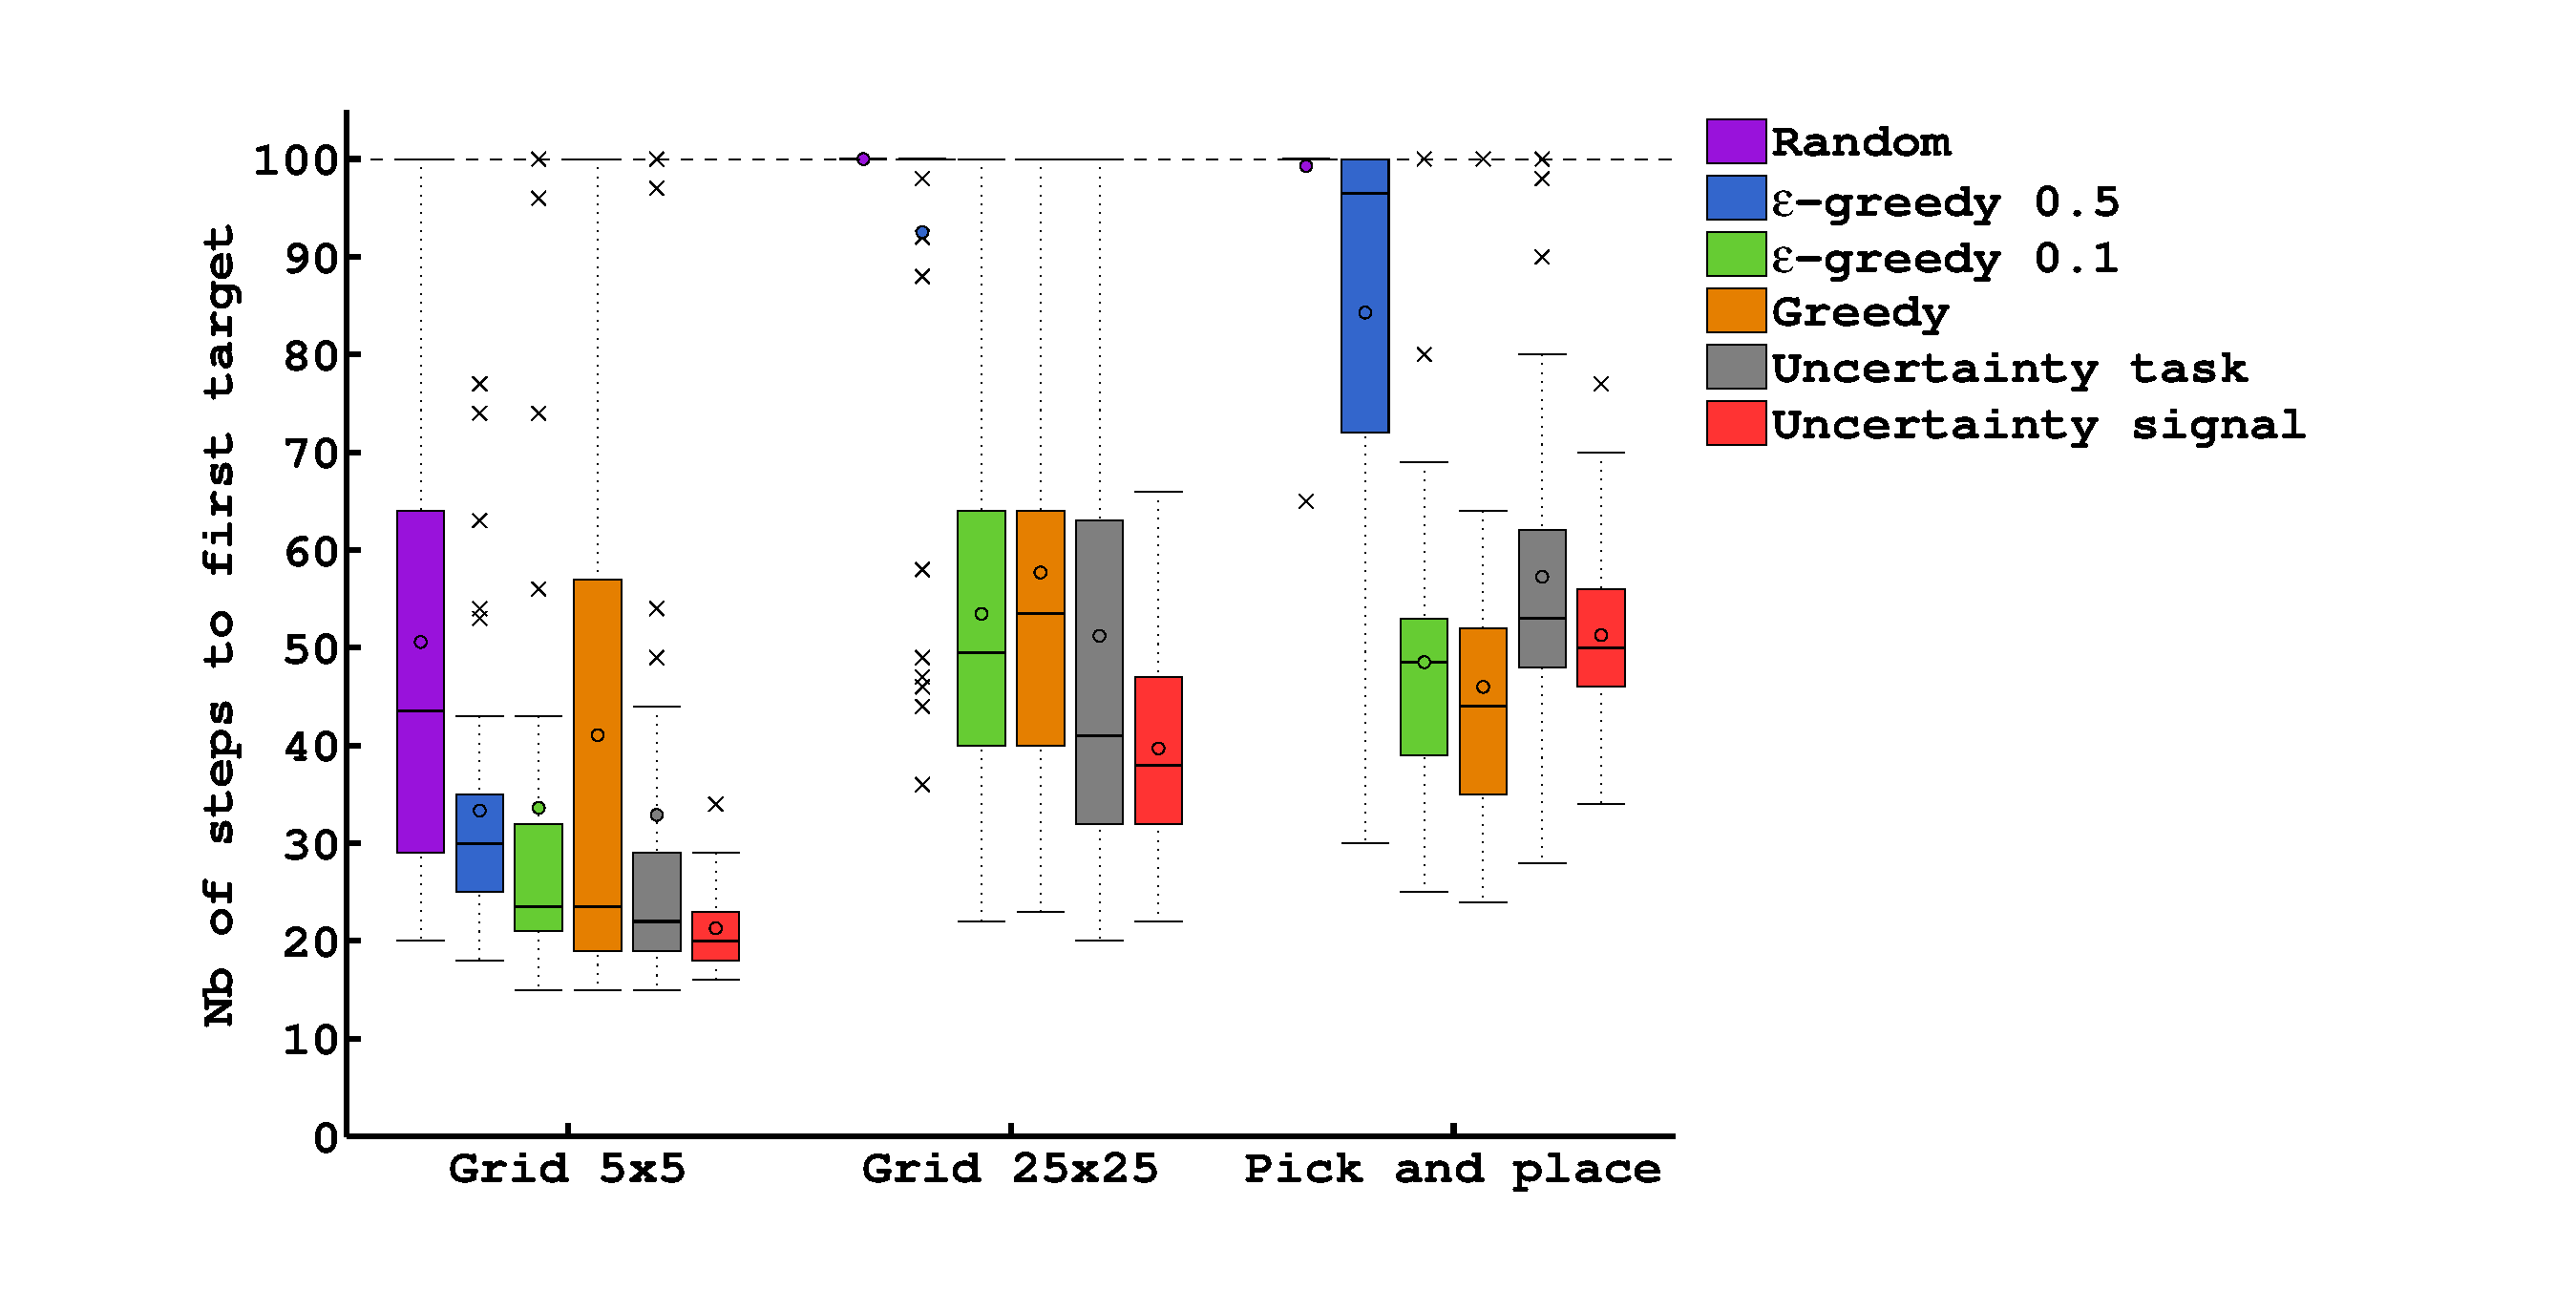
\includegraphics[width=\legendsidesize\columnwidth]{\imgpath/world_properties/firstreach.eps}
\caption{Number of steps to reach first target state with confidence.}
\label{fig:wordlpropertiestimefirst}
\end{figure}

We report only 9 erroneous first task estimations across all runs of our experiments and conditions.For the grid world, 1 error for the Greedy method in. For the pick and place scenario, 1 for $\epsilon$-greedy 0.5, 2 for $\epsilon$-greedy 0.1, 2 for Greedy, 1 for Uncertainty task and 2 for Uncertainty signal.

\begin{table}[!ht]
\centering
\rowcolors{2}{gray!25}{white}
\begin{tabular}{c c c c}
    Planning method & Gridworld 25x25 &  Pick and place \\ \hline
    Random & 0 & 1 \\ 
    $\epsilon$-greedy 0.5 & 13 & 27 \\
    $\epsilon$-greedy 0.1 & 48 & 48 \\
    Greedy & 43 & 47 \\
    Uncertainty task & 42 & 48 \\
    Uncertainty signal & 50 & 50 \\
\end{tabular}
\caption{Number of experiments that reached at least one target in 100 steps.}
\label{tab:}
\end{table}

\begin{figure}[!ht]
\centering
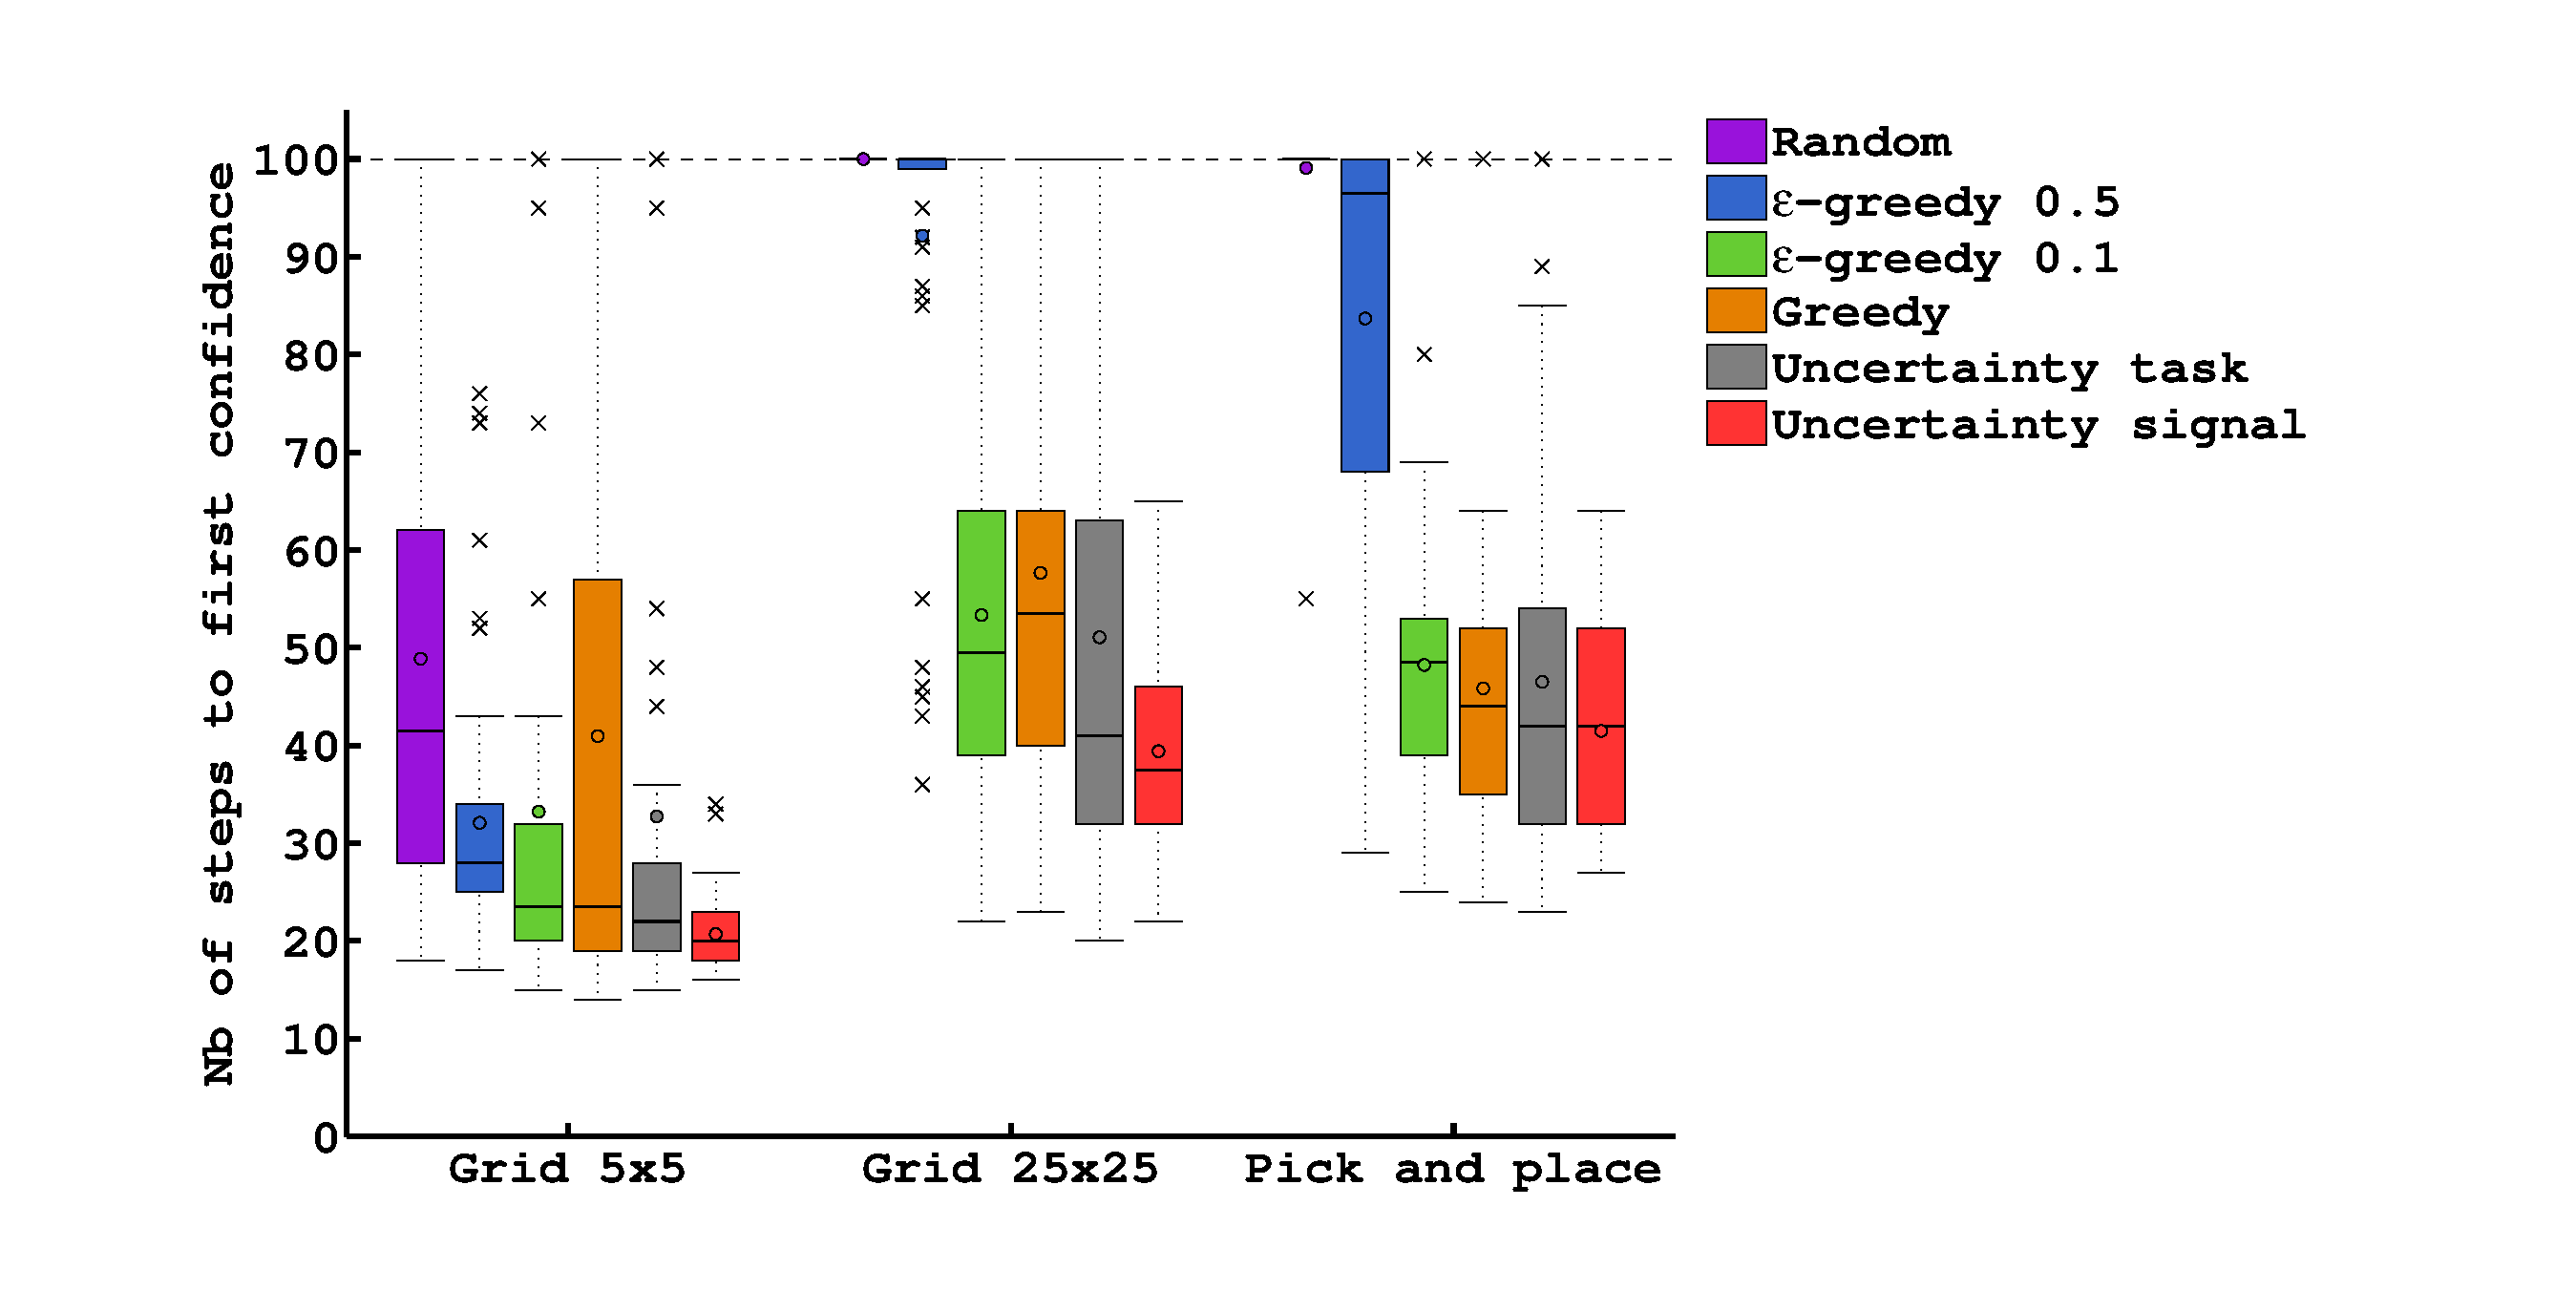
\includegraphics[width=\legendsidesize\columnwidth]{\imgpath/world_properties/firstconfident.eps}
\caption{Number of steps to reach confidence level for the first target.}
\label{fig:wordlpropertiesconfidencefirst}
\end{figure} 

\begin{figure}[!ht]
\centering
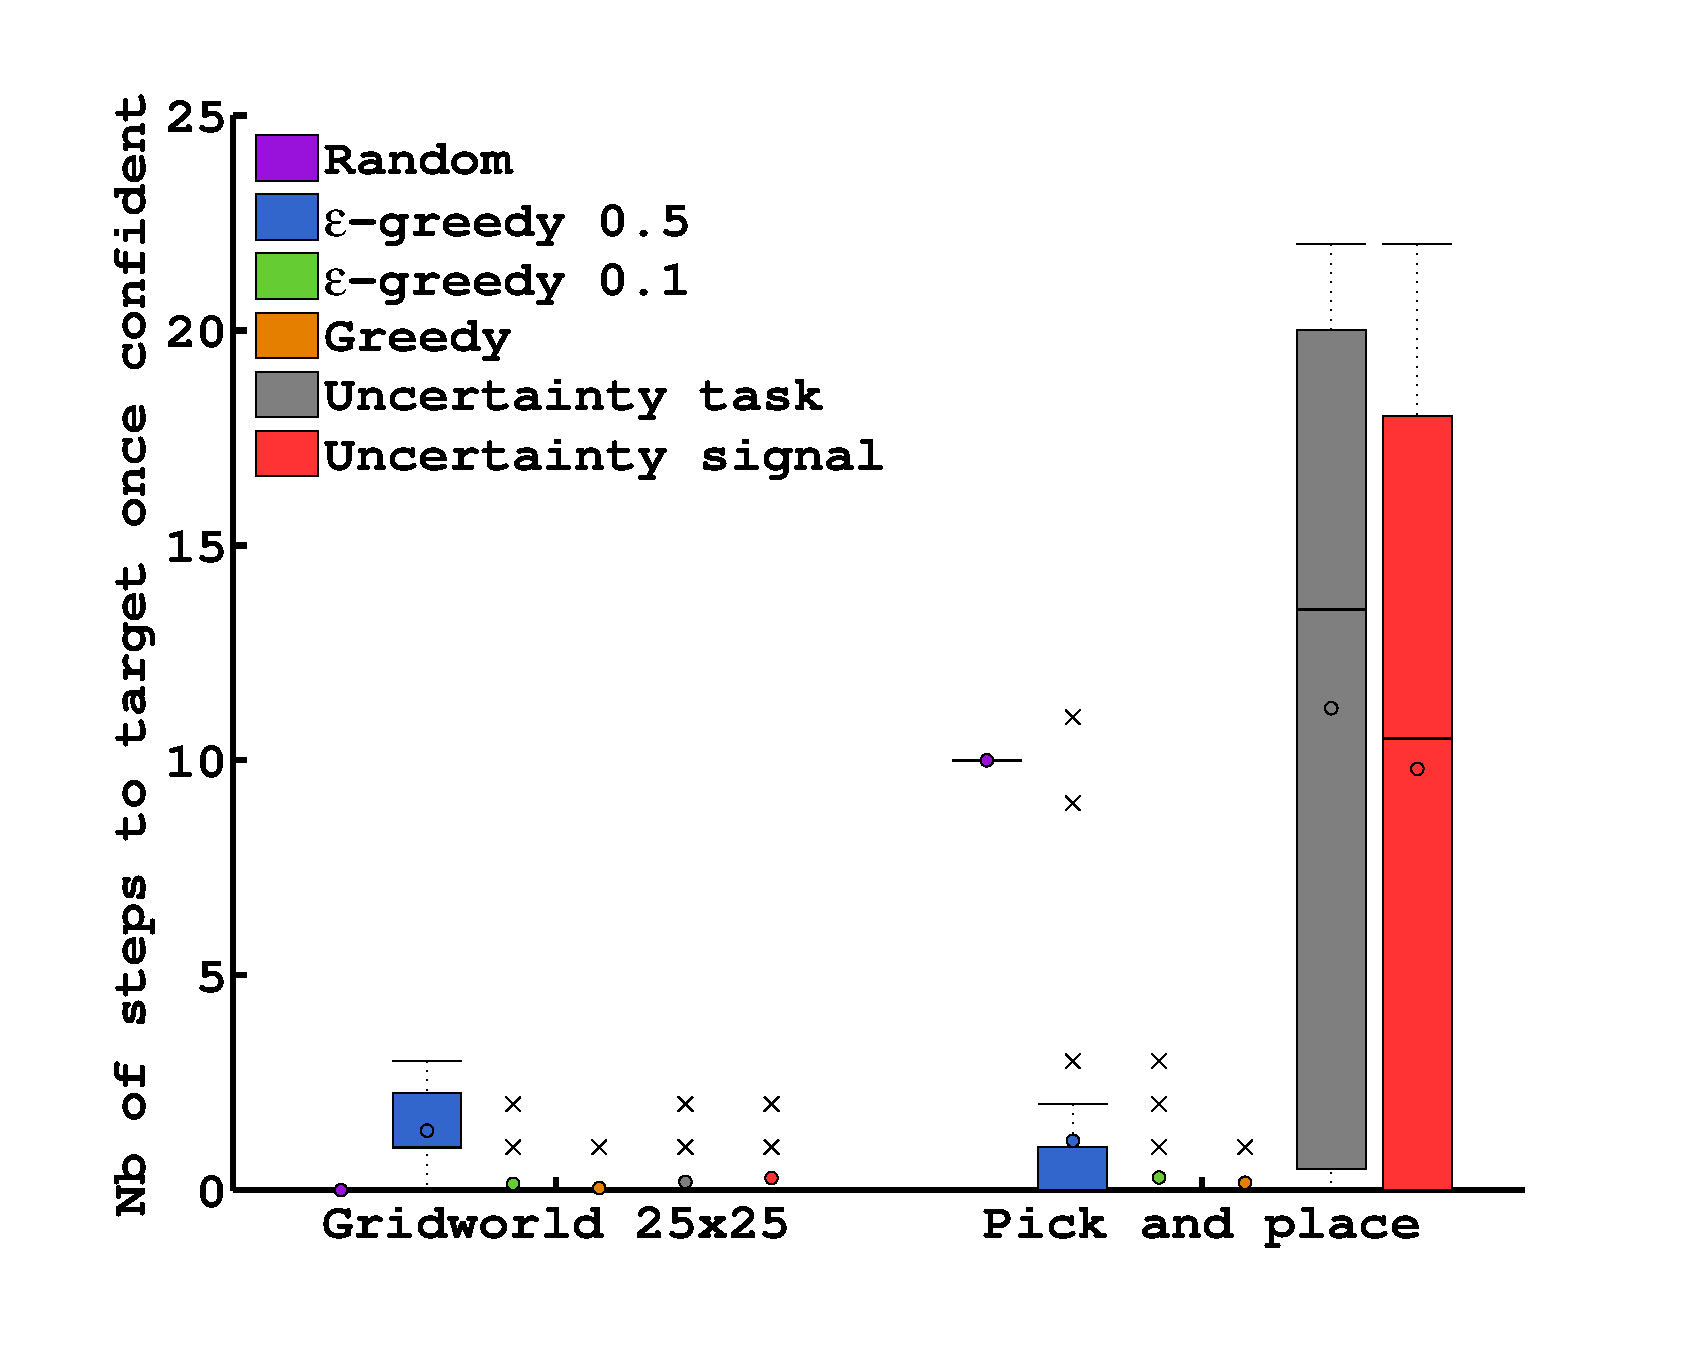
\includegraphics[width=\plotsize\columnwidth]{\imgpath/world_properties/difftargetconfidence.eps}
\caption{Number of action needed to reach the first target when the agent reach confidence level for this target.}
\label{fig:wordlpropertiestargetdist}
\end{figure} 

refer to experiment with pick and place in section lfui and random planning (even if dataset the same after 100 step no confidence) but state space is 625 and no ore 25...
random after 100 not at the confident level.


\subsection{Discussion}

it is obviously dependent on plenty of other things not tested here the frame and signals quality and stuff

should we compare on the number of state or on the number of state action pair?

conclude by stating difference between end goal learning (graps object, reach state) and reward based learning. We only consider goal learning. episodic (find the right box) vs endless (collect more reward), different exploration function could be used for those

